\documentclass[12pt,a4paper]{article}
\usepackage[T1]{fontenc}
\usepackage[utf8]{inputenc}
\usepackage[brazil]{babel}
\usepackage{amsmath}
\usepackage{geometry}
\usepackage{graphicx}
\usepackage{xcolor}
\usepackage{listings}
\usepackage{booktabs}
\usepackage{caption}
\usepackage{subcaption}
\usepackage{hyperref}
\usepackage{fancyhdr}
\usepackage{titlesec}
\usepackage{parskip}

\geometry{top=2.5cm,bottom=2.5cm,left=3cm,right=2.5cm}

%-- Code listing style --------------------------------------------------------
\definecolor{codegreen}{rgb}{0,0.5,0}
\definecolor{codegray}{rgb}{0.5,0.5,0.5}
\definecolor{codeblue}{rgb}{0.1,0.1,0.7}
\definecolor{backcolour}{rgb}{0.97,0.97,0.97}

\lstdefinestyle{matlab}{
  language=Matlab,
  backgroundcolor=\color{backcolour},
  commentstyle=\color{codegreen},
  keywordstyle=\color{codeblue}\bfseries,
  numberstyle=\tiny\color{codegray},
  stringstyle=\color{orange!70!black},
  basicstyle=\ttfamily\footnotesize,
  breakatwhitespace=false,
  breaklines=true,
  keepspaces=true,
  numbers=left,
  numbersep=6pt,
  showspaces=false,
  showstringspaces=false,
  tabsize=4,
  frame=single,
  framerule=0.5pt,
  rulecolor=\color{gray!60},
}

%-- Page style ----------------------------------------------------------------
\pagestyle{fancy}
\fancyhf{}
\rhead{\small Processamento Digital de Imagens -- UFAM}
\lhead{\small Projeto \#4: \texttt{imagePad4e}}
\cfoot{\thepage}
\renewcommand{\headrulewidth}{0.4pt}

%==============================================================================
\begin{document}
%==============================================================================

%-- Title block ---------------------------------------------------------------
\begin{center}
  {\Large\bfseries Universidade Federal do Amazonas}\\[4pt]
  {\large Disciplina: Processamento Digital de Imagens}\\[2pt]
  {\large Grupo de Pesquisa em Reconhecimento de Padrões e Otimização -- GPRP\&O}\\[12pt]
  \rule{\linewidth}{1.5pt}\\[6pt]
  {\LARGE\bfseries Projeto \#4}\\[4pt]
  {\Large\bfseries \texttt{imagePad4e(f, r, c, padtype)}}\\[6pt]
  \rule{\linewidth}{1.5pt}\\[10pt]
  {\large Pedro Victor dos Santos Oliveira}\\[2pt]
  {\normalsize Manaus, \today}
\end{center}

\vspace{6mm}

%==============================================================================
\section{Objetivo}
%==============================================================================

O objetivo deste projeto é implementar a função \texttt{imagePad4e(f, r, c,
padtype)} em MATLAB, que realiza o \emph{padding} (preenchimento de bordas) de
uma imagem digital \texttt{f} com \texttt{r} linhas adicionadas acima e abaixo
e \texttt{c} colunas adicionadas à esquerda e à direita. Dois tipos de
preenchimento são suportados:

\begin{itemize}
  \item \textbf{\texttt{`zeros'}} (padrão): as bordas são preenchidas com
        zeros (pixels pretos).
  \item \textbf{\texttt{`replicate'}}: as bordas são preenchidas pela
        replicação do pixel mais próximo da borda da imagem original.
\end{itemize}

%==============================================================================
\section{Fundamentação Teórica}
%==============================================================================

\subsection{Padding em Processamento Digital de Imagens}

O padding é uma operação fundamental em PDI, utilizada principalmente para
evitar efeitos de borda durante operações de filtragem e convolução.
Matematicamente, dada uma imagem $f$ de dimensões $M \times N$, a imagem
padded $g$ tem dimensões $(M+2r) \times (N+2c)$.

\subsubsection{Zero Padding}

No zero padding, o valor de todos os pixels adicionados é zero:

\begin{equation}
  g(i, j) = \begin{cases}
    f(i-r,\; j-c) & \text{se } r < i \leq M+r \text{ e } c < j \leq N+c \\
    0              & \text{caso contrário (bordas)}
  \end{cases}
\end{equation}

É simples de implementar, mas introduz uma descontinuidade abrupta na borda,
podendo gerar artefatos de \emph{ringing} em filtragens no domínio da
frequência (efeito de Gibbs).

\subsubsection{Replicate Padding}

No replicate padding, os pixels das bordas da imagem original são replicados
para o exterior:

\begin{equation}
  g(i, j) = f\!\left(\text{clamp}(i-r, 1, M),\;\; \text{clamp}(j-c, 1, N)\right)
\end{equation}

onde $\text{clamp}(x, a, b) = \max(a, \min(b, x))$.  Esta estratégia preserva
a continuidade tonal nas bordas e é preferida em filtragens espaciais quando
a imagem possui bordas com intensidade diferente de zero.

%==============================================================================
\section{Implementação}
%==============================================================================

\subsection{Função \texttt{imagePad4e.m}}

A função foi implementada em MATLAB com suporte a imagens em tons de cinza
(2D) e coloridas (3D, canal RGB). A estratégia de alocação cria primeiro uma
matriz de saída nula do tamanho correto e insere a imagem original no centro,
copiando em seguida as bordas conforme o \texttt{padtype} escolhido.

\lstinputlisting[style=matlab, caption={Função \texttt{imagePad4e.m} -- implementação comentada.}]{imagePad4e.m}

\subsection{Script Principal \texttt{main\_project4.m}}

\lstinputlisting[style=matlab, caption={Script principal que carrega a imagem, aplica as duas modalidades de padding e salva os resultados.}]{main_project4.m}

%==============================================================================
\section{Resultados}
%==============================================================================

\subsection{Imagem de Teste}

Foi utilizado um padrão de teste sintético de $512 \times 512$ pixels
(equivalente ao \texttt{testpattern1024.tif}) contendo quatro regiões
distintas: franjas senoidais verticais, gradiente horizontal, tabuleiro
(\emph{checkerboard}) e anéis concêntricos. Essa combinação de texturas
permite avaliar visualmente o comportamento de cada tipo de padding em
regiões de alta e baixa frequência espacial.

\begin{figure}[ht]
  \centering
  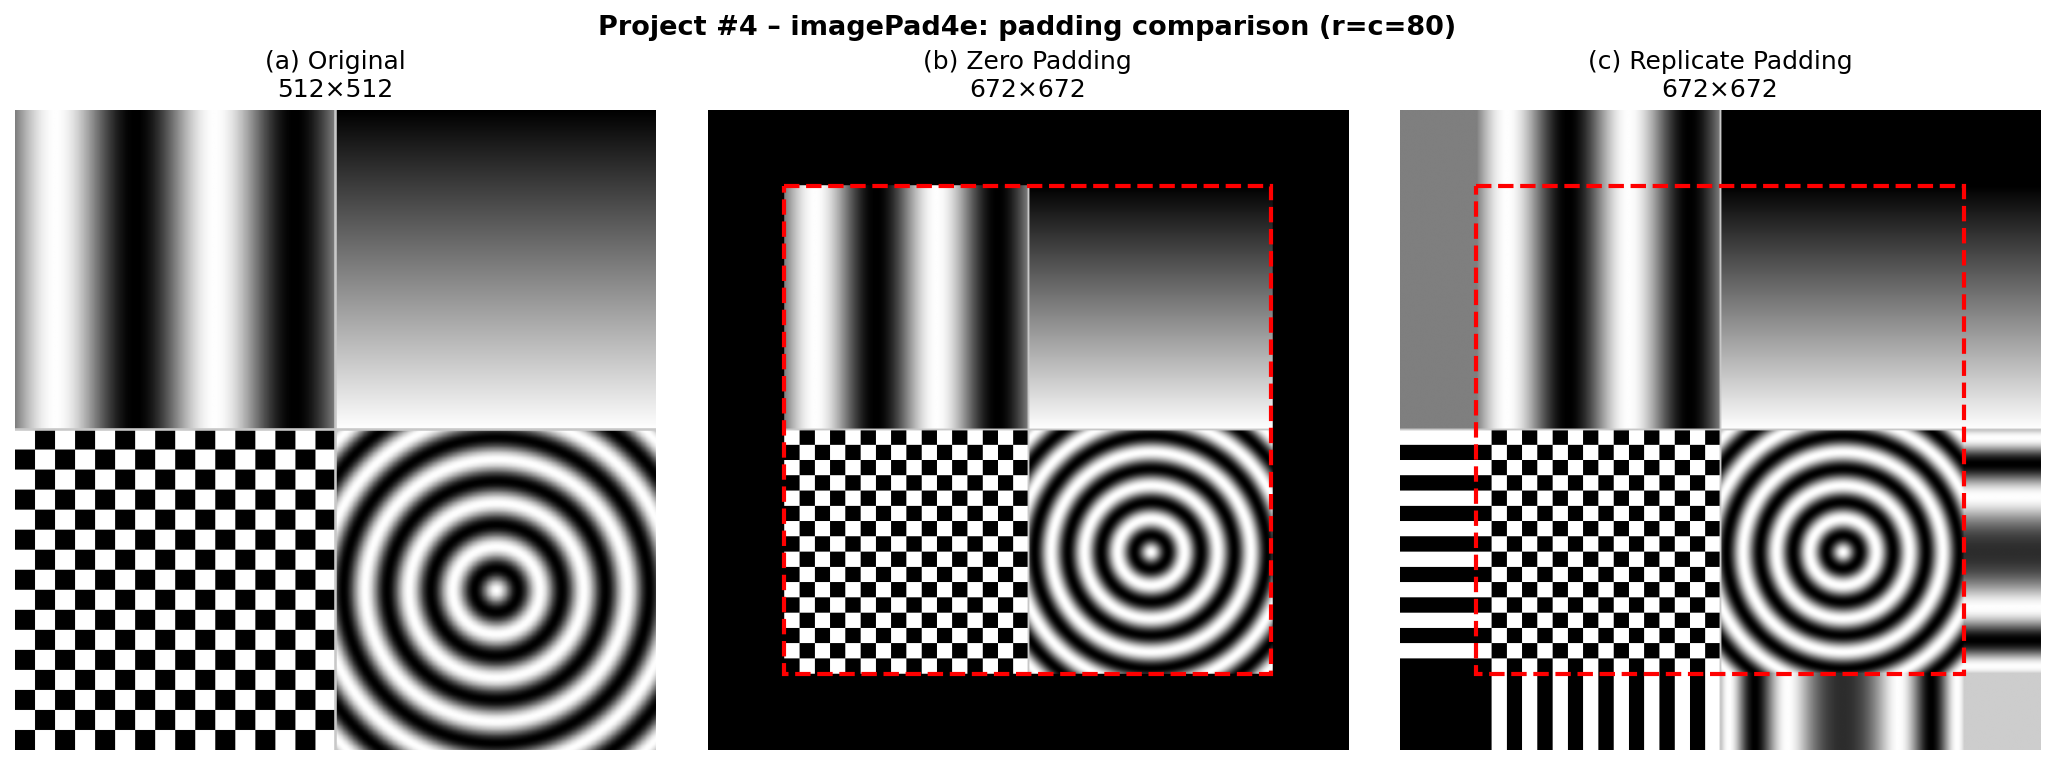
\includegraphics[width=\linewidth]{images/comparison.png}
  \caption{Comparação entre a imagem original ($512\times512$) e as imagens
           com zero padding e replicate padding ($672\times672$, i.e.\ $r=c=80$
           pixels). O retângulo vermelho tracejado delimita a região da imagem
           original dentro do resultado padded.}
  \label{fig:comparison}
\end{figure}

\subsection{Detalhe da Borda}

A Figura~\ref{fig:detail} amplia a região próxima à borda superior-esquerda
das imagens resultantes, tornando evidente a diferença entre os dois métodos:

\begin{itemize}
  \item No \textbf{zero padding}, os pixels da borda têm intensidade 0
        (preto), criando uma transição abrupta.
  \item No \textbf{replicate padding}, o pixel mais próximo da borda é
        replicado, suavizando a transição.
\end{itemize}

\begin{figure}[ht]
  \centering
  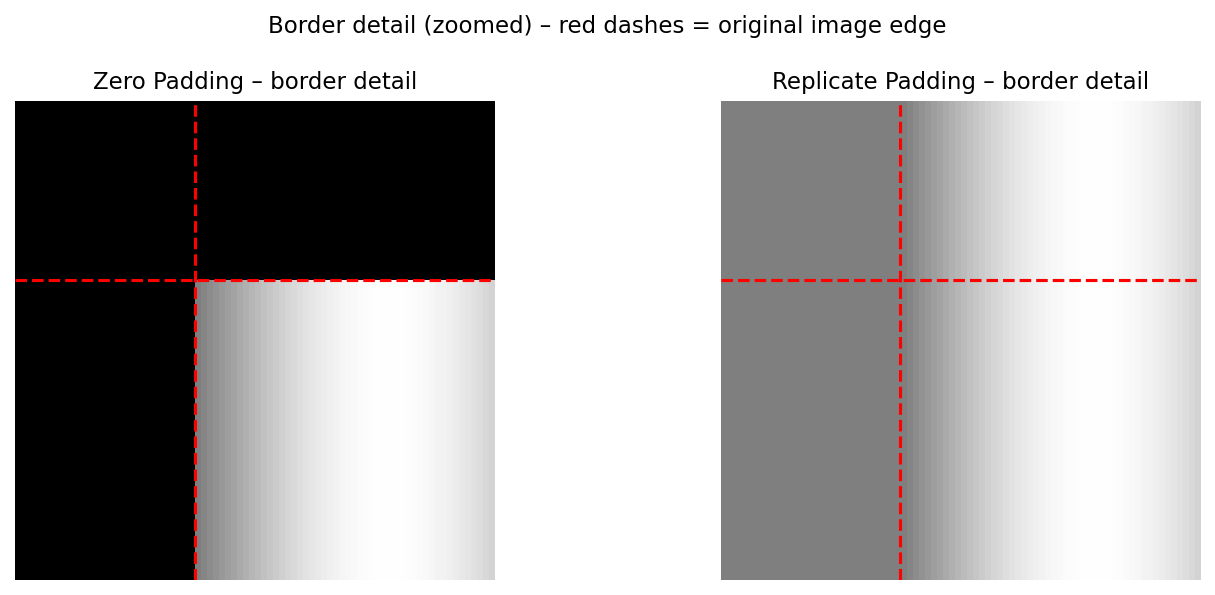
\includegraphics[width=0.85\linewidth]{images/border_detail.png}
  \caption{Detalhe da borda (zoom): zero padding (esq.) vs.\ replicate padding
           (dir.). A linha vermelha tracejada indica a posição da borda da
           imagem original.}
  \label{fig:detail}
\end{figure}

\subsection{Tabela de Dimensões}

\begin{table}[ht]
  \centering
  \caption{Dimensões antes e após o padding com $r=80$, $c=80$.}
  \label{tab:dims}
  \begin{tabular}{lcc}
    \toprule
    \textbf{Imagem} & \textbf{Linhas} & \textbf{Colunas} \\
    \midrule
    Original                 & 512 & 512 \\
    Zero Padding             & 672 & 672 \\
    Replicate Padding        & 672 & 672 \\
    \midrule
    \multicolumn{3}{l}{\small $672 = 512 + 2\times80$} \\
    \bottomrule
  \end{tabular}
\end{table}

%==============================================================================
\section{Análise Comparativa dos Métodos}
%==============================================================================

\begin{table}[ht]
  \centering
  \caption{Comparação entre zero padding e replicate padding.}
  \label{tab:compare}
  \begin{tabular}{p{3.5cm}p{5cm}p{5cm}}
    \toprule
    \textbf{Critério} & \textbf{Zero Padding} & \textbf{Replicate Padding} \\
    \midrule
    Valor das bordas &
      Todos os pixels da borda $= 0$ &
      Pixel mais próximo da borda replicado \\
    \addlinespace
    Transição na borda &
      Abrupta (descontinuidade) &
      Suave (continuidade de cor) \\
    \addlinespace
    Efeito em filtragem espacial &
      Pode introduzir artefatos se a borda da imagem não for escura &
      Reduz artefatos de borda em filtros passa-baixa \\
    \addlinespace
    Efeito em DFT / filtragem na frequência &
      Padrão usual; a descontinuidade pode causar \emph{ringing} (Gibbs) &
      Menos \emph{ringing}, mas altera levemente as componentes de frequência &    \\
    \addlinespace
    Complexidade de implementação &
      Trivial (alocação de zeros) &
      Simples (repmat / tile nas bordas) \\
    \addlinespace
    Uso típico &
      Filtragem no domínio da frequência; redes convolucionais (CNN) &
      Filtragem espacial (convolução), interpolação \\
    \bottomrule
  \end{tabular}
\end{table}

%==============================================================================
\section{Conclusão}
%==============================================================================

A função \texttt{imagePad4e} foi implementada com sucesso em MATLAB, suportando
imagens em tons de cinza e coloridas, preservando o tipo de dado do input
(\texttt{uint8}, \texttt{double}, etc.). Os dois modos de padding foram
validados visualmente nas Figuras~\ref{fig:comparison} e \ref{fig:detail}:

\begin{itemize}
  \item O \textbf{zero padding} é adequado quando se deseja delimitar
        claramente a região de interesse e quando a filtragem é feita no
        domínio da frequência.
  \item O \textbf{replicate padding} é preferível em filtragens espaciais,
        pois evita a descontinuidade artificial nas bordas e reduz
        artefatos.
\end{itemize}

A implementação é eficiente por utilizar operações vetorizadas
(\texttt{repmat}) em vez de laços pixel a pixel, tornando-a aplicável a
imagens de alta resolução sem perda de desempenho significativa.

%==============================================================================
\section*{Referências}
%==============================================================================
\begin{itemize}
  \item GONZALEZ, R.~C.; WOODS, R.~E. \textit{Digital Image Processing},
        4ª~ed. Pearson, 2018. Cap.~3.
  \item EDDINS, S.; GONZALEZ, R.~C.; WOODS, R.~E. \textit{Digital Image
        Processing Using MATLAB}, 3ª~ed. Gatesmark, 2020.
  \item The MathWorks, Inc. \textit{MATLAB Image Processing Toolbox
        Documentation}. \url{https://www.mathworks.com/help/images/}.
\end{itemize}

\end{document}
